% Options for packages loaded elsewhere
\PassOptionsToPackage{unicode}{hyperref}
\PassOptionsToPackage{hyphens}{url}
%
\documentclass[
]{article}
\usepackage{lmodern}
\usepackage{amsmath}
\usepackage{ifxetex,ifluatex}
\ifnum 0\ifxetex 1\fi\ifluatex 1\fi=0 % if pdftex
  \usepackage[T1]{fontenc}
  \usepackage[utf8]{inputenc}
  \usepackage{textcomp} % provide euro and other symbols
  \usepackage{amssymb}
\else % if luatex or xetex
  \usepackage{unicode-math}
  \defaultfontfeatures{Scale=MatchLowercase}
  \defaultfontfeatures[\rmfamily]{Ligatures=TeX,Scale=1}
\fi
% Use upquote if available, for straight quotes in verbatim environments
\IfFileExists{upquote.sty}{\usepackage{upquote}}{}
\IfFileExists{microtype.sty}{% use microtype if available
  \usepackage[]{microtype}
  \UseMicrotypeSet[protrusion]{basicmath} % disable protrusion for tt fonts
}{}
\makeatletter
\@ifundefined{KOMAClassName}{% if non-KOMA class
  \IfFileExists{parskip.sty}{%
    \usepackage{parskip}
  }{% else
    \setlength{\parindent}{0pt}
    \setlength{\parskip}{6pt plus 2pt minus 1pt}}
}{% if KOMA class
  \KOMAoptions{parskip=half}}
\makeatother
\usepackage{xcolor}
\IfFileExists{xurl.sty}{\usepackage{xurl}}{} % add URL line breaks if available
\IfFileExists{bookmark.sty}{\usepackage{bookmark}}{\usepackage{hyperref}}
\hypersetup{
  pdftitle={Economic scarring in Sheffield \& Rotherham},
  pdfauthor={Dan Olner},
  hidelinks,
  pdfcreator={LaTeX via pandoc}}
\urlstyle{same} % disable monospaced font for URLs
\usepackage[margin=1in]{geometry}
\usepackage{graphicx}
\makeatletter
\def\maxwidth{\ifdim\Gin@nat@width>\linewidth\linewidth\else\Gin@nat@width\fi}
\def\maxheight{\ifdim\Gin@nat@height>\textheight\textheight\else\Gin@nat@height\fi}
\makeatother
% Scale images if necessary, so that they will not overflow the page
% margins by default, and it is still possible to overwrite the defaults
% using explicit options in \includegraphics[width, height, ...]{}
\setkeys{Gin}{width=\maxwidth,height=\maxheight,keepaspectratio}
% Set default figure placement to htbp
\makeatletter
\def\fps@figure{htbp}
\makeatother
\setlength{\emergencystretch}{3em} % prevent overfull lines
\providecommand{\tightlist}{%
  \setlength{\itemsep}{0pt}\setlength{\parskip}{0pt}}
\setcounter{secnumdepth}{-\maxdimen} % remove section numbering
\usepackage{dcolumn}
\ifluatex
  \usepackage{selnolig}  % disable illegal ligatures
\fi

\title{Economic scarring in Sheffield \& Rotherham}
\author{Dan Olner}
\date{22/04/2022}

\begin{document}
\maketitle

Our analysis of scarring in Sheffield uses several ideas from a paper by
Patricia Rice and Anthony Venables (Rice \& Venables 2021), in which
they explore how the effect of economic shocks in the 1970s are still
affecting Great Britain today. Here, we are able to use much a
finer-grained geography, allowing us to examine employment change
\emph{within} areas, rather than just comparing areas. The top-level
geographies we use are \textbf{travel to work areas (TTWA)}: each of
these zones aims to capture the majority of commuting happening within
that zone - they tend to centre on major towns and cities, and include
their surrounding commute areas. Below this level - for example, when
looking at Sheffield and Rotherham in detail - we use \textbf{electoral
wards}.

The decade from 1971 to 1981 saw employment decrease in every single
TTWA in Great Britain. As Rice \& Venables note, ``It is not the case
that the LADs that suffered the largest negative employment shocks in
the 1970s were performing poorly in 1971'' (p.133). This is certainly
true for Sheffield. To give an overview of the employment change pattern
from 1971 to 2011, and how Sheffield fits into that pattern, figure 1
plots the employment percentage in ten TTWAs - plus Sheffield \&
Rotherham - in each of the five Census decades in our data. It picks out
five TTWAs that saw the largest drops in employment between 1971 to 1981
(in red) and the small drops (in blue). The red TTWAs are examples of
the point Rice \& Venables make: many areas in Great Britain that had
very high employment levels in 1971 were hit hardest in the subsequent
ten years, seeing huge changes in their employment fortunes. Sheffield
is closer to one of these type of areas - strong employment in 1971, hit
very hard.

Note, however, how all the TTWAs in this figure with the largest
employment decrease from 1971 to 1981 (in red) `bounce back' in 1981 to
1991. This is what Rice \& Venables suggest should be expected if there
is no economic `scarring': adjustment should take place through, for
example, migration - both internal within Great Britain, and via non-UK
migrants moving to areas - leading to employment equilibrium,
geographically (ibid p.134). However, almost exactly fifty percent of
Great Britain's TTWAs saw their employment \emph{drop} from 1981 to
1991; Sheffield is part of a cluster of areas that suffered from this
two-decade-long economic decline, as can be seen in figure 1.

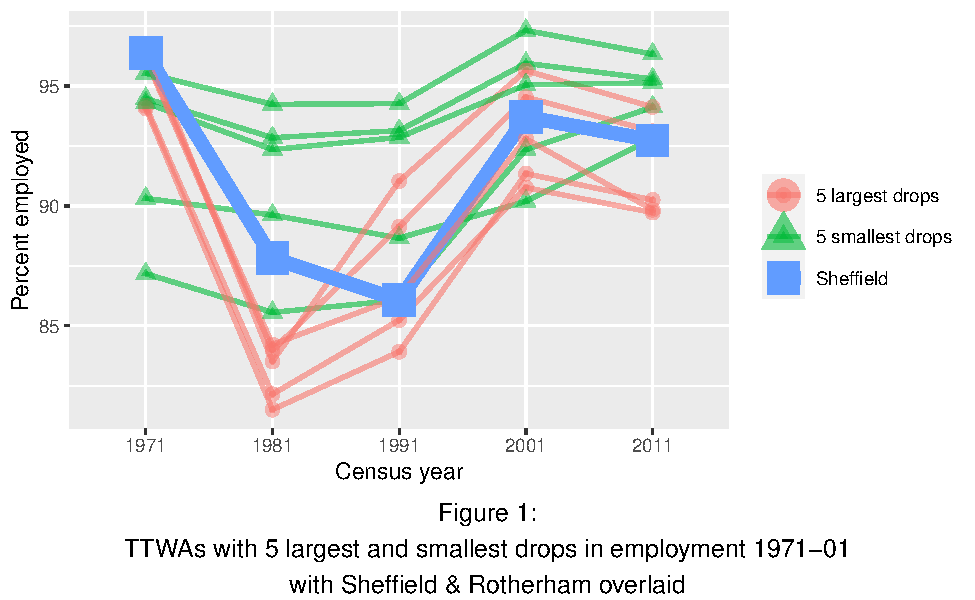
\includegraphics{SheffieldScarring_Writeup1_Apr2022_files/figure-latex/unnamed-chunk-2-1.pdf}

Figure 2 shows the raw employment percent numbers for each of the more
than ten thousand wards in Great Britain, with one Census on the x axis
and the subsequent decade on the y axis. A line of slope 1 passing
through zero is overlaid in green, and Sheffield \& Rotherham's wards
are overlaid in red. Figure 2(a) shows the change between 1971 and 1981:
any wards below the slope line had higher employment in 1971 than 1981:
very few gained in that decade, and it is clear that all of Sheffield's
wards were affected by the shock more strongly than others (they are at
the lower side of the plot). Figure 2(b) shows the same for the
transition in employment from 1981 to 1991, a decade later: the slope
line divides wards fairly evenly between those that gained employment
within that decade and those that lost - supporting the point above that
around 50\% of areas saw employment drop for a further decade. The
majority of Sheffield's wards are on the lower side of the line - their
employment level dropped again - though there are four to five wards
that gained a little.

{[}Seems to me useful to include these before the slightly more abstract
use of ``difference from average emlpoyment ppt per Census''{]}

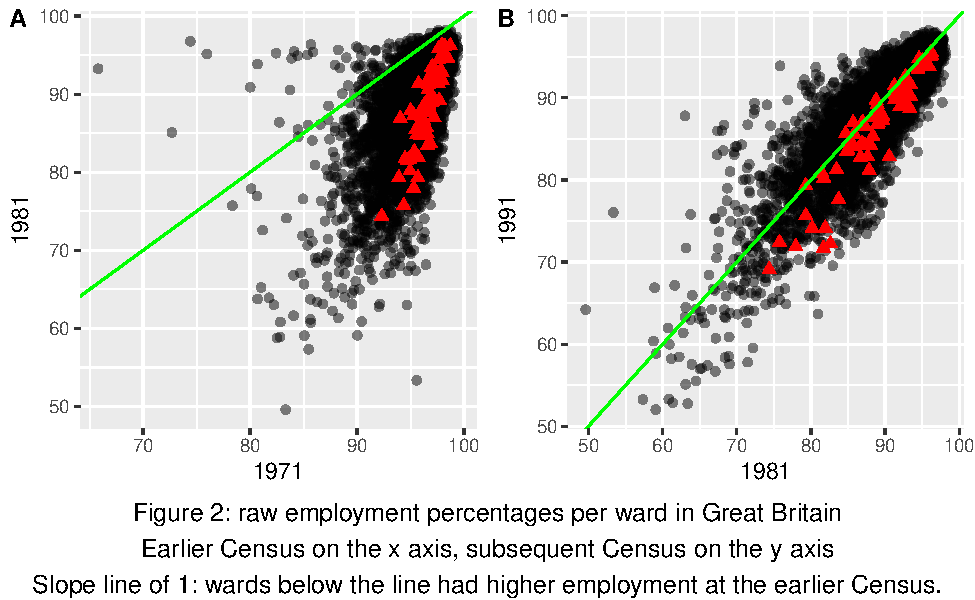
\includegraphics{SheffieldScarring_Writeup1_Apr2022_files/figure-latex/unnamed-chunk-3-1.pdf}

Rice \& Venables find a persistent effect of the 1971-81 shock on
employment levels in later decades at local authority scale across
England and Wales. There are two aspects of their analysis that we
re-create here at the smaller ward scale of Sheffield and Rotherham.
First, we use the \textbf{percentage point difference from the average
employment rate at each Census} (we label this the \textbf{employment
rate (ER)}: this makes cross-Census comparisons easier. Second, we then
find how ER \emph{changes} between different Censuses and use this to
compare how employment changed between 1971-1981 (the economic shock
period) and other time periods.

The argument Rice \& Venables makes is as follows: if places were not
economically scarred by the 1971-81 shock, `one wou'convergence' would
be expected:

\begin{quote}
``The classic (or neoclassical) forces for convergence are simply that
wage adjustment will cause some combination of replacement jobs moving
into adversely affected places, and population moving out.'' (p.134)
\end{quote}

They use change of ER betwewen Census periods to examine whether this
happened by comparing two time periods to the `shock' decade of 1971-81.
Correlating the shock change to 1971 to 2011 - overlapping the same time
period - gives an indication as to whether the shock impacts persisted
to the most recent census. A positive correlation would be expected if
they did. the shock period is also compared to the whole period
\emph{after} 1981 (so, correlating 1971-81 with 1981-2011): if
convergence had taken place, there would be `bounceback': a negative
correlation as employment reverts some way to its previous level.

Rice \& venables find no convergence in the latter period. However, when
looking at the sub-regional scale of wards, some convergence can be
found. Figure 3 shows this for Sheffield \& Rotherham. Figure 3(a)
examines 1971-81 versus 1971-2011: the positive slope indicates
persistence of the 1971-81 shock. Conversely, figure 3(b) has a negative
slope, showing there was some bounceback for Sheffield wards in the
latter time period. Note, this is not true for all wards however: the
zero axes are marked to help make this clear, with two examples in the
plots. The Sheffield ward marked as a blue triangle is in the bottom
left quadrant for the 1971-81 versus 1971-11 comparison in 3(a), but in
the top left quadrant in 3(b): while that ward dropped relative to other
wards in the shock period, it bounced back in the latter period. In
contrast, the ward marked with a red square is in the bottom left of
both plots: it dropped relative to other wards in all examined time
periods, seeing less bounceback (it is slightly less negative in the
latter period).

Overall, then, there is evidence of convergence - but not for very ward
within Sheffield \& Rotherham and, as shown above, Sheffield was
relatively worse off after the shock than many other areas.

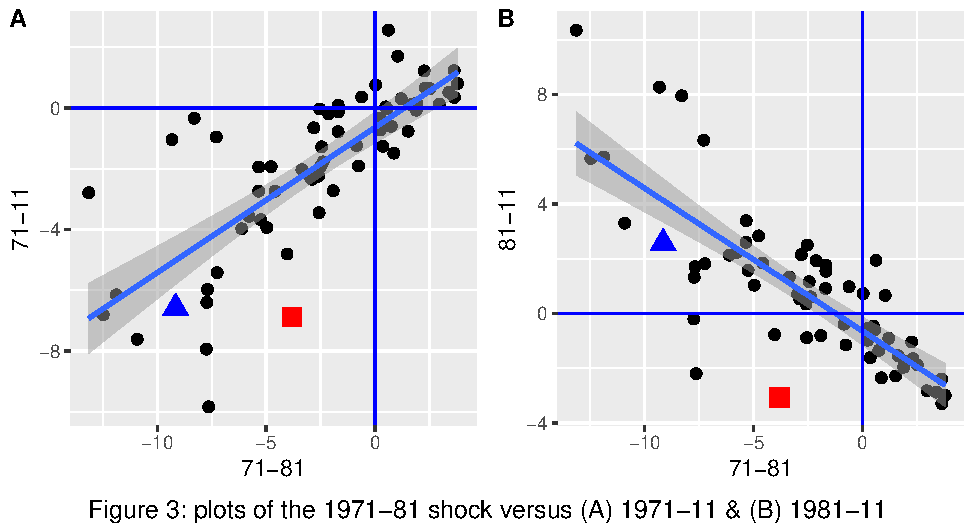
\includegraphics{SheffieldScarring_Writeup1_Apr2022_files/figure-latex/unnamed-chunk-4-1.pdf}

We examine this further by using the same variables in figure 3 for a
set of regressions, with the 1971-81 shock period's change in ER as the
main predictor variable and a series of different time periods as the
outcome. We include a second predictor: the percentage of non-UK-born
people in each ward in 1971, also interacting this with the 71-81 shock
predictor. Here, we are asking: if there was a high migrant population
in an area in 1971, did that have a protective or exacerbating effect on
employment change?

We include three sets of identical regressions for different
geographies: first for Great Britain as a whole, then Sheffield \&
Rotherham, and - for reasons explained below - London. As well as
regressions for the correlations examined in figure 3, the other outcome
periods included are each subsequent decade: 1981-91, 1991-2001 and
2001-2011. These are included to examine the full pattern of how the
71-81 shock period affected later decades.

Each regression table shows the pattern identified above: persistence of
the shock through the entire 1971-2011 period (positive coefficients for
the `71-81' predictor in column 1, matching the slope in figure 3a) and
a bounceback effect for 1981-2011 (column 2's negative coeffients).

For Great Britain as a whole (table 1), for both the 71-11 and 81-11
periods, the non-UK-born coefficient is negative. Specifically, for
every 10\% increase in non-UK-born, 71-11 and 81-11 change decreases by
0.4 percentage points: places with a higher non-UK-born proportion saw a
larger relative drop. The interaction term for Great Britain shows how
much the 71-81 predictor's slope changes as a result of a 1 unit change
in non-UK-born proportion. While it is positive here, the effect size is
small, making any conclusions from the interaction tenuous.

Sheffield \& Rotherham (table) certainly see the 1971-81 shock impact in
columns 1 and 2: there is a larger initial shock value, and a smaller
bounceback coefficient in column 2, confirming the plots above. The lack
of significance of the non-UK-born coefficient is likely due to the much
smaller number of wards in this area compared to Great Britain.

Even, though it cannot be seen clearly for Sheffield, does the Great
Britain result mean non-UK-born people were having a negative effect on
the employment shock? One problem with this conclusion is that, when
examining the whole of Great Britain, no distinction is made between
urban and rural areas. It is urban areas where the 1971-81 shock was
primarily felt - and these are also the places where migrants would go
to find work. The positive coefficient may just be reflecting this
urban/rural split: more migrants lived in places hardest hit.

To test this, the same regressions for London are also included (table
3). The whole London TTWA is mostly urban, and it has always had a large
non-UK-born population. Any migrant impacts \emph{within} London should
be able to test for an urban/rural effect. As can be seen in columns 1
and 2 for the non-UK-born coefficient, a 10\% increase in non-UK-born is
associated with a nearly one-percent-point increase in 71-11 and 81-11
ER change. In contrast to Great Britain as a whole, places with a higher
perentage non-UK-born in London did better in terms of employment
impacts from the shock. This supports the theory that the difference in
Great Britain as a whole is due to the urban/rural split.

\begin{table}[!htbp] \centering 
  \caption{Great Britain} 
  \label{} 
\begin{tabular}{@{\extracolsep{5pt}}lD{.}{.}{-3} D{.}{.}{-3} D{.}{.}{-3} D{.}{.}{-3} D{.}{.}{-3} } 
\\[-1.8ex]\hline 
\hline \\[-1.8ex] 
 & \multicolumn{5}{c}{\textit{Dependent variable:}} \\ 
\cline{2-6} 
\\[-1.8ex] & \multicolumn{1}{c}{`71-11`} & \multicolumn{1}{c}{`81-11`} & \multicolumn{1}{c}{`81-91`} & \multicolumn{1}{c}{`91-01`} & \multicolumn{1}{c}{`01-11`} \\ 
\\[-1.8ex] & \multicolumn{1}{c}{(1)} & \multicolumn{1}{c}{(2)} & \multicolumn{1}{c}{(3)} & \multicolumn{1}{c}{(4)} & \multicolumn{1}{c}{(5)}\\ 
\hline \\[-1.8ex] 
 `71-81` & 0.333^{***} & -0.667^{***} & -0.190^{***} & -0.527^{***} & 0.050^{***} \\ 
  & (0.006) & (0.006) & (0.007) & (0.006) & (0.004) \\ 
  & & & & & \\ 
 nonUK\_pc71 & -0.042^{***} & -0.042^{***} & -0.142^{***} & 0.084^{***} & 0.017^{***} \\ 
  & (0.004) & (0.004) & (0.005) & (0.004) & (0.003) \\ 
  & & & & & \\ 
 `71-81`:nonUK\_pc71 & 0.004^{***} & 0.004^{***} & 0.010^{***} & -0.001^{*} & -0.005^{***} \\ 
  & (0.001) & (0.001) & (0.001) & (0.001) & (0.001) \\ 
  & & & & & \\ 
 Constant & 0.196^{***} & 0.196^{***} & 0.661^{***} & -0.385^{***} & -0.081^{***} \\ 
  & (0.028) & (0.028) & (0.033) & (0.028) & (0.018) \\ 
  & & & & & \\ 
\hline \\[-1.8ex] 
Observations & \multicolumn{1}{c}{10,180} & \multicolumn{1}{c}{10,180} & \multicolumn{1}{c}{10,180} & \multicolumn{1}{c}{10,180} & \multicolumn{1}{c}{10,180} \\ 
R$^{2}$ & \multicolumn{1}{c}{0.353} & \multicolumn{1}{c}{0.639} & \multicolumn{1}{c}{0.151} & \multicolumn{1}{c}{0.553} & \multicolumn{1}{c}{0.022} \\ 
Adjusted R$^{2}$ & \multicolumn{1}{c}{0.353} & \multicolumn{1}{c}{0.639} & \multicolumn{1}{c}{0.151} & \multicolumn{1}{c}{0.553} & \multicolumn{1}{c}{0.022} \\ 
Residual Std. Error (df = 10176) & \multicolumn{1}{c}{2.108} & \multicolumn{1}{c}{2.108} & \multicolumn{1}{c}{2.484} & \multicolumn{1}{c}{2.125} & \multicolumn{1}{c}{1.382} \\ 
F Statistic (df = 3; 10176) & \multicolumn{1}{c}{1,853.419$^{***}$} & \multicolumn{1}{c}{6,005.614$^{***}$} & \multicolumn{1}{c}{602.792$^{***}$} & \multicolumn{1}{c}{4,203.178$^{***}$} & \multicolumn{1}{c}{76.816$^{***}$} \\ 
\hline 
\hline \\[-1.8ex] 
\textit{Note:}  & \multicolumn{5}{r}{$^{*}$p$<$0.1; $^{**}$p$<$0.05; $^{***}$p$<$0.01} \\ 
\end{tabular} 
\end{table}

\begin{table}[!htbp] \centering 
  \caption{Sheffield/Rotherham} 
  \label{} 
\begin{tabular}{@{\extracolsep{5pt}}lD{.}{.}{-3} D{.}{.}{-3} D{.}{.}{-3} D{.}{.}{-3} D{.}{.}{-3} } 
\\[-1.8ex]\hline 
\hline \\[-1.8ex] 
 & \multicolumn{5}{c}{\textit{Dependent variable:}} \\ 
\cline{2-6} 
\\[-1.8ex] & \multicolumn{1}{c}{`71-11`} & \multicolumn{1}{c}{`81-11`} & \multicolumn{1}{c}{`81-91`} & \multicolumn{1}{c}{`91-01`} & \multicolumn{1}{c}{`01-11`} \\ 
\\[-1.8ex] & \multicolumn{1}{c}{(1)} & \multicolumn{1}{c}{(2)} & \multicolumn{1}{c}{(3)} & \multicolumn{1}{c}{(4)} & \multicolumn{1}{c}{(5)}\\ 
\hline \\[-1.8ex] 
 `71-81` & 0.454^{***} & -0.546^{***} & 0.031 & -0.625^{***} & 0.048 \\ 
  & (0.087) & (0.087) & (0.112) & (0.093) & (0.072) \\ 
  & & & & & \\ 
 nonUK\_pc71 & 0.059 & 0.059 & 0.035 & -0.067 & 0.091 \\ 
  & (0.173) & (0.173) & (0.223) & (0.185) & (0.143) \\ 
  & & & & & \\ 
 `71-81`:nonUK\_pc71 & 0.011 & 0.011 & 0.060^{*} & -0.028 & -0.022 \\ 
  & (0.028) & (0.028) & (0.036) & (0.030) & (0.023) \\ 
  & & & & & \\ 
 Constant & -0.750^{*} & -0.750^{*} & -1.473^{***} & 0.952^{**} & -0.229 \\ 
  & (0.418) & (0.418) & (0.538) & (0.448) & (0.347) \\ 
  & & & & & \\ 
\hline \\[-1.8ex] 
Observations & \multicolumn{1}{c}{64} & \multicolumn{1}{c}{64} & \multicolumn{1}{c}{64} & \multicolumn{1}{c}{64} & \multicolumn{1}{c}{64} \\ 
R$^{2}$ & \multicolumn{1}{c}{0.587} & \multicolumn{1}{c}{0.629} & \multicolumn{1}{c}{0.213} & \multicolumn{1}{c}{0.730} & \multicolumn{1}{c}{0.089} \\ 
Adjusted R$^{2}$ & \multicolumn{1}{c}{0.567} & \multicolumn{1}{c}{0.610} & \multicolumn{1}{c}{0.174} & \multicolumn{1}{c}{0.716} & \multicolumn{1}{c}{0.044} \\ 
Residual Std. Error (df = 60) & \multicolumn{1}{c}{1.761} & \multicolumn{1}{c}{1.761} & \multicolumn{1}{c}{2.266} & \multicolumn{1}{c}{1.886} & \multicolumn{1}{c}{1.461} \\ 
F Statistic (df = 3; 60) & \multicolumn{1}{c}{28.458$^{***}$} & \multicolumn{1}{c}{33.844$^{***}$} & \multicolumn{1}{c}{5.419$^{***}$} & \multicolumn{1}{c}{53.954$^{***}$} & \multicolumn{1}{c}{1.957} \\ 
\hline 
\hline \\[-1.8ex] 
\textit{Note:}  & \multicolumn{5}{r}{$^{*}$p$<$0.1; $^{**}$p$<$0.05; $^{***}$p$<$0.01} \\ 
\end{tabular} 
\end{table}

\begin{table}[!htbp] \centering 
  \caption{London} 
  \label{} 
\begin{tabular}{@{\extracolsep{5pt}}lD{.}{.}{-3} D{.}{.}{-3} D{.}{.}{-3} D{.}{.}{-3} D{.}{.}{-3} } 
\\[-1.8ex]\hline 
\hline \\[-1.8ex] 
 & \multicolumn{5}{c}{\textit{Dependent variable:}} \\ 
\cline{2-6} 
\\[-1.8ex] & \multicolumn{1}{c}{`71-11`} & \multicolumn{1}{c}{`81-11`} & \multicolumn{1}{c}{`81-91`} & \multicolumn{1}{c}{`91-01`} & \multicolumn{1}{c}{`01-11`} \\ 
\\[-1.8ex] & \multicolumn{1}{c}{(1)} & \multicolumn{1}{c}{(2)} & \multicolumn{1}{c}{(3)} & \multicolumn{1}{c}{(4)} & \multicolumn{1}{c}{(5)}\\ 
\hline \\[-1.8ex] 
 `71-81` & 0.538^{***} & -0.462^{***} & 0.382^{***} & -0.775^{***} & -0.069^{***} \\ 
  & (0.034) & (0.034) & (0.043) & (0.029) & (0.025) \\ 
  & & & & & \\ 
 nonUK\_pc71 & 0.085^{***} & 0.085^{***} & -0.047^{***} & 0.055^{***} & 0.077^{***} \\ 
  & (0.006) & (0.006) & (0.008) & (0.005) & (0.005) \\ 
  & & & & & \\ 
 `71-81`:nonUK\_pc71 & -0.005^{**} & -0.005^{**} & 0.0001 & -0.002 & -0.002 \\ 
  & (0.002) & (0.002) & (0.002) & (0.002) & (0.001) \\ 
  & & & & & \\ 
 Constant & -2.815^{***} & -2.815^{***} & -2.360^{***} & 0.471^{***} & -0.925^{***} \\ 
  & (0.104) & (0.104) & (0.130) & (0.089) & (0.077) \\ 
  & & & & & \\ 
\hline \\[-1.8ex] 
Observations & \multicolumn{1}{c}{962} & \multicolumn{1}{c}{962} & \multicolumn{1}{c}{962} & \multicolumn{1}{c}{962} & \multicolumn{1}{c}{962} \\ 
R$^{2}$ & \multicolumn{1}{c}{0.396} & \multicolumn{1}{c}{0.556} & \multicolumn{1}{c}{0.272} & \multicolumn{1}{c}{0.753} & \multicolumn{1}{c}{0.305} \\ 
Adjusted R$^{2}$ & \multicolumn{1}{c}{0.394} & \multicolumn{1}{c}{0.555} & \multicolumn{1}{c}{0.269} & \multicolumn{1}{c}{0.753} & \multicolumn{1}{c}{0.303} \\ 
Residual Std. Error (df = 958) & \multicolumn{1}{c}{1.861} & \multicolumn{1}{c}{1.861} & \multicolumn{1}{c}{2.335} & \multicolumn{1}{c}{1.589} & \multicolumn{1}{c}{1.384} \\ 
F Statistic (df = 3; 958) & \multicolumn{1}{c}{209.409$^{***}$} & \multicolumn{1}{c}{400.589$^{***}$} & \multicolumn{1}{c}{119.115$^{***}$} & \multicolumn{1}{c}{975.662$^{***}$} & \multicolumn{1}{c}{140.400$^{***}$} \\ 
\hline 
\hline \\[-1.8ex] 
\textit{Note:}  & \multicolumn{5}{r}{$^{*}$p$<$0.1; $^{**}$p$<$0.05; $^{***}$p$<$0.01} \\ 
\end{tabular} 
\end{table}

Lastly, we examine whether the 1971-81 shock had a lasting effect on
deprivation in Sheffield and Rotherham. To do this, we re-create a
figure from Rice \& Venables: this plots employment percentages in 2011
against deprivation rank, and overlays what we label the `shock decile'.
This puts all wards into a decile based on how negative the effect of
the 1971-81 shock was on their ED. Wards in decile 1 were the worst
affected. The plot marks wards in deciles 1 and 2, thus showing where
those worst impacted in 1971-81 found themselves in the 2019 deprivation
rank.

For the deprivation rank itself, we use the 2019 English indices of
deprivation (ONS 2019), finding the population-weighted average
deprivation score per ward before re-ranking. In figure 4, this rank is
on the y axis: lower values at the bottom are more deprived wards.

The plot includes both Sheffield \& Rotherham and London, for
comparison. Shock decile 1 wards (the worst impacted in 1971-81) are
shown in red circles; decile 2 (second-worst) are green triangles. It is
clear that Sheffield \& Rotherham wards worst affected in 1971-81 have
both lower employment levels in 2011, and are more deprived than others
in the region. The graph for London confirms this pattern is repeated.

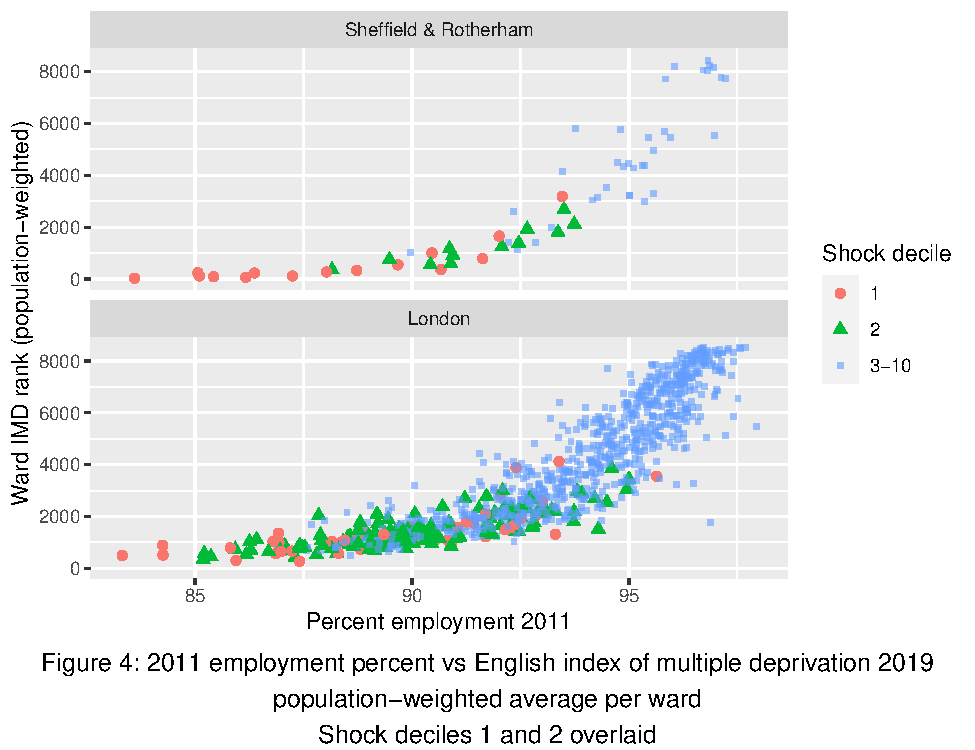
\includegraphics{SheffieldScarring_Writeup1_Apr2022_files/figure-latex/unnamed-chunk-10-1.pdf}

\end{document}
